

\section{Appendix: Parametrization of anomalous couplings in dijet \texorpdfstring{$p_T$}{pT}}
%%%%%%%%%%%%%%%%%%%%%%%%%%%%
%%%%%%%%%%%%%%%%%%%%%%%%%%%%
We parametrize the ratio of dijet $p_T$ spectrum 
for anomalous coupling events with respect to the 
SM prediction shown in 
Figs.~\ref{fig:ww_dijetPt_atgcRatio06}-\ref{fig:ww_dijetPt_atgcRatio004}.
The functional form used is
%%%%%%%%%%%
\begin{equation}
\text{Ratio} = p0 + p1 \cdot x + p2 \cdot x^2,
\end{equation}
%%%%%%%%%%%
where the variable $x$ is dijet $p_T$ and 
$p0$, $p1$, and $p2$ are constant parameters.


\subsection{Variation in \texorpdfstring{$\Lambda_Z$}{LambdaZ}}
Below are the values of $p0$, $p1$, and $p2$ 
for samples where $\Lambda_Z$ is varied 
while $\Delta{\kappa_\gamma} = 0$.

\begin{verbatim}
LambdaZ = 0.6, deltaKappaGamma=0
--------------------------------
Chi2                      =      3.64986
NDf                       =           11
p0                        =      11.2278   +/-   2.81571     
p1                        =    -0.223741   +/-   0.0399655   
p2                        =   0.00123161   +/-   0.00011465  

LambdaZ = 0.4, deltaKappaGamma=0
--------------------------------
Chi2                      =      1.42274
NDf                       =           11
p0                        =      5.95071   +/-   2.31201     
p1                        =     -0.10545   +/-   0.0307862   
p2                        =  0.000565467   +/-   8.47447e-05 

LambdaZ = 0.36, deltaKappaGamma=0
--------------------------------
Chi2                      =      1.12979
NDf                       =           11
p0                        =      5.12598   +/-   2.20968     
p1                        =   -0.0872118   +/-   0.0289282   
p2                        =  0.000463317   +/-   7.87343e-05 

LambdaZ = 0.32, deltaKappaGamma=0
--------------------------------
Chi2                      =     0.897387
NDf                       =           11
p0                        =      4.43249   +/-   2.11338     
p1                        =   -0.0715905   +/-   0.0271381   
p2                        =  0.000374281   +/-   7.29155e-05 

LambdaZ = 0.28, deltaKappaGamma=0
--------------------------------
Chi2                      =     0.918216
NDf                       =           11
p0                        =      4.17028   +/-   2.04504     
p1                        =   -0.0656265   +/-   0.0259669   
p2                        =  0.000335899   +/-   6.93965e-05 

LambdaZ = 0.24, deltaKappaGamma=0
--------------------------------
Chi2                      =     0.529841
NDf                       =           11
p0                        =      3.02472   +/-   1.91317     
p1                        =   -0.0418764   +/-   0.0234578   
p2                        =  0.000215939   +/-   6.09107e-05 

LambdaZ = 0.20, deltaKappaGamma=0
--------------------------------

Chi2                      =     0.402117
NDf                       =           11
p0                        =      2.44186   +/-   1.81022     
p1                        =   -0.0298704   +/-   0.0215866   
p2                        =  0.000152795   +/-   5.48662e-05 

LambdaZ = 0.16, deltaKappaGamma=0
--------------------------------
Chi2                      =     0.352723
NDf                       =           11
p0                        =      1.89519   +/-   1.70728     
p1                        =    -0.018908   +/-   0.0196807   
p2                        =   9.7063e-05   +/-   4.86507e-05 

LambdaZ = 0.12, deltaKappaGamma=0
--------------------------------
Chi2                      =     0.280284
NDf                       =           11
p0                        =      1.10707   +/-   1.53445     
p1                        =  -0.00557192   +/-   0.0172814   
p2                        =  3.87113e-05   +/-   4.14116e-05 

LambdaZ = 0.08, deltaKappaGamma=0
--------------------------------
Chi2                      =      1.04598
NDf                       =           11
p0                        =      0.87561   +/-   1.44635     
p1                        = -0.000634317   +/-   0.0155036   
p2                        =  1.23603e-05   +/-   3.56521e-05 

LambdaZ = 0.04, deltaKappaGamma=0
--------------------------------
Chi2                      =      1.03194
NDf                       =           11
p0                        =     0.792353   +/-   1.31868     
p1                        =  0.000442174   +/-   0.0135901   
p2                        =  3.28419e-06   +/-   3.03898e-05 

LambdaZ = -0.04, deltaKappaGamma=0
----------------------------------
Chi2                      =     0.388485
NDf                       =           11
p0                        =      1.17295   +/-   1.41256     
p1                        =  -0.00312795   +/-   0.0140684   
p2                        =  9.69201e-06   +/-   3.08623e-05 


LambdaZ = -0.08, deltaKappaGamma=0
----------------------------------
Chi2                      =     0.224663
NDf                       =           11
p0                        =     0.992352   +/-   1.42183     
p1                        =  -0.00270947   +/-   0.0149806   
p2                        =  1.59717e-05   +/-   3.41951e-05 

LambdaZ = -0.12, deltaKappaGamma=0
----------------------------------
Chi2                      =      1.09498
NDf                       =           11
p0                        =     0.748711   +/-   1.5101      
p1                        =  -0.00123123   +/-   0.0168109   
p2                        =   2.6301e-05   +/-   3.96608e-05 

LambdaZ = -0.16, deltaKappaGamma=0
----------------------------------
Chi2                      =     0.318396
NDf                       =           11
p0                        =      1.98487   +/-   1.66882     
p1                        =   -0.0205248   +/-   0.0191608   
p2                        =  9.86346e-05   +/-   4.74287e-05 

LambdaZ = -0.20, deltaKappaGamma=0
----------------------------------
Chi2                      =      0.38124
NDf                       =           11
p0                        =      2.46184   +/-   1.76528     
p1                        =   -0.0301792   +/-   0.020942    
p2                        =  0.000148224   +/-   5.32002e-05 


LambdaZ = -0.24, deltaKappaGamma=0
----------------------------------
Chi2                      =     0.521923
NDf                       =           11
p0                        =      3.05575   +/-   1.86202     
p1                        =    -0.042438   +/-   0.022743    
p2                        =  0.000211166   +/-   5.91106e-05 

LambdaZ = -0.28, deltaKappaGamma=0
----------------------------------
Chi2                      =     0.716835
NDf                       =           11
p0                        =      3.72376   +/-   1.95772     
p1                        =   -0.0565562   +/-   0.0245455   
p2                        =  0.000285148   +/-   6.50602e-05 

LambdaZ = -0.32, deltaKappaGamma=0
----------------------------------
Chi2                      =      0.93626
NDf                       =           11
p0                        =      4.43248   +/-   2.05067     
p1                        =   -0.0718192   +/-   0.0263008   
p2                        =  0.000366903   +/-   7.08617e-05 

LambdaZ = -0.36, deltaKappaGamma=0
----------------------------------
Chi2                      =      1.19243
NDf                       =           11
p0                        =      5.18671   +/-   2.14791     
p1                        =    -0.088321   +/-   0.0281072   
p2                        =  0.000457363   +/-   7.67586e-05 


LambdaZ = -0.40, deltaKappaGamma=0
----------------------------------
Chi2                      =      1.47664
NDf                       =           11
p0                        =      5.98969   +/-   2.24334     
p1                        =    -0.106212   +/-   0.0298892   
p2                        =  0.000557032   +/-   8.25968e-05 

LambdaZ = -0.60, deltaKappaGamma=0
----------------------------------
Chi2                      =      3.75932
NDf                       =           11
p0                        =      11.0856   +/-   2.72881     
p1                        =    -0.221749   +/-   0.0388708   
p2                        =   0.00120986   +/-   0.000112021 
\end{verbatim}


\subsection{Variation in \texorpdfstring{$\Delta{\kappa_\gamma}$}{deltaKappaGamma}}
Below are the values of $p0$, $p1$, and $p2$ 
for samples where $\Delta{\kappa_\gamma}$ is varied 
while $\Lambda_Z = 0$.


\begin{verbatim}
LambdaZ = 0.0, deltaKappaGamma=0.6
----------------------------------
Chi2                      =     0.299454
NDf                       =           11
p0                        =      1.86622   +/-   1.66398     
p1                        =   -0.0183681   +/-   0.0190694   
p2                        =  9.01579e-05   +/-   4.69879e-05 

LambdaZ = 0.0, deltaKappaGamma=0.4
----------------------------------
Chi2                      =     0.160771
NDf                       =           11
p0                        =      1.44302   +/-   1.56269     
p1                        =  -0.00785653   +/-   0.016885    
p2                        =  3.57502e-05   +/-   3.95597e-05 

LambdaZ = 0.0, deltaKappaGamma=0.2
----------------------------------
Chi2                      =     0.190735
NDf                       =           11
p0                        =      1.02335   +/-   1.41674     
p1                        =  -0.00197093   +/-   0.014597    
p2                        =   1.0576e-05   +/-   3.27614e-05 

LambdaZ = 0.0, deltaKappaGamma=-0.2
----------------------------------
Chi2                      =     0.233846
NDf                       =           11
p0                        =       1.0455   +/-   1.39176     
p1                        =  -0.00291274   +/-   0.0145155   
p2                        =  1.38214e-05   +/-   3.29594e-05 

LambdaZ = 0.0, deltaKappaGamma=-0.4
----------------------------------
Chi2                      =     0.254044
NDf                       =           11
p0                        =      1.15303   +/-   1.5165      
p1                        =  -0.00592117   +/-   0.0166971   
p2                        =  3.58467e-05   +/-   3.95137e-05 

LambdaZ = 0.0, deltaKappaGamma=-0.6
------------------------------------
Chi2                      =     0.323557
NDf                       =           11
p0                        =       1.7774   +/-   1.71582     
p1                        =   -0.0171167   +/-   0.0198797   
p2                        =   9.3204e-05   +/-   4.91357e-05 
\end{verbatim}


\subsection{Parametrization of ratio}
Finally, we write the ratio of dijet $p_T$ spectrum 
with respect to the SM prediction as 
%%%%%%%%%%%
\begin{equation}
\text{Ratio} = \text{constant term} + 
\text{linear term} \cdot x + \text{quadratic term} \cdot x^2,
\label{eqatgcparam}
\end{equation}
%%%%%%%%%%%
where the variable $x$ is dijet $p_T$ and 
the three coefficients are quadratic functions of 
the anomalous coupling value.
%%%%%%%%%%%
\begin{equation}
\text{Each coefficient in Eq.~\ref{eqatgcparam}} = a0 + a1 \cdot aTGC + a2 \cdot aTGC^2.
\end{equation}
%%%%%%%%%%%
Parameters $a0$, $a1$, $a2$ are listed 
below for $\Lambda_Z$ and $\Delta{\kappa_\gamma}$.
Each coefficient in Eq.~\ref{eqatgcparam} 
is also  shown in Fig.~\ref{fig:aTGC_parametrization} 
as a function of the anomalous coupling.
%%%%%%%%%%%%%%%%%%%%%%%%%%%%
%%%%%%%%%%%%%%%%%%%%%%%%%%%%
\begin{figure}[h!t]
  {\centering
    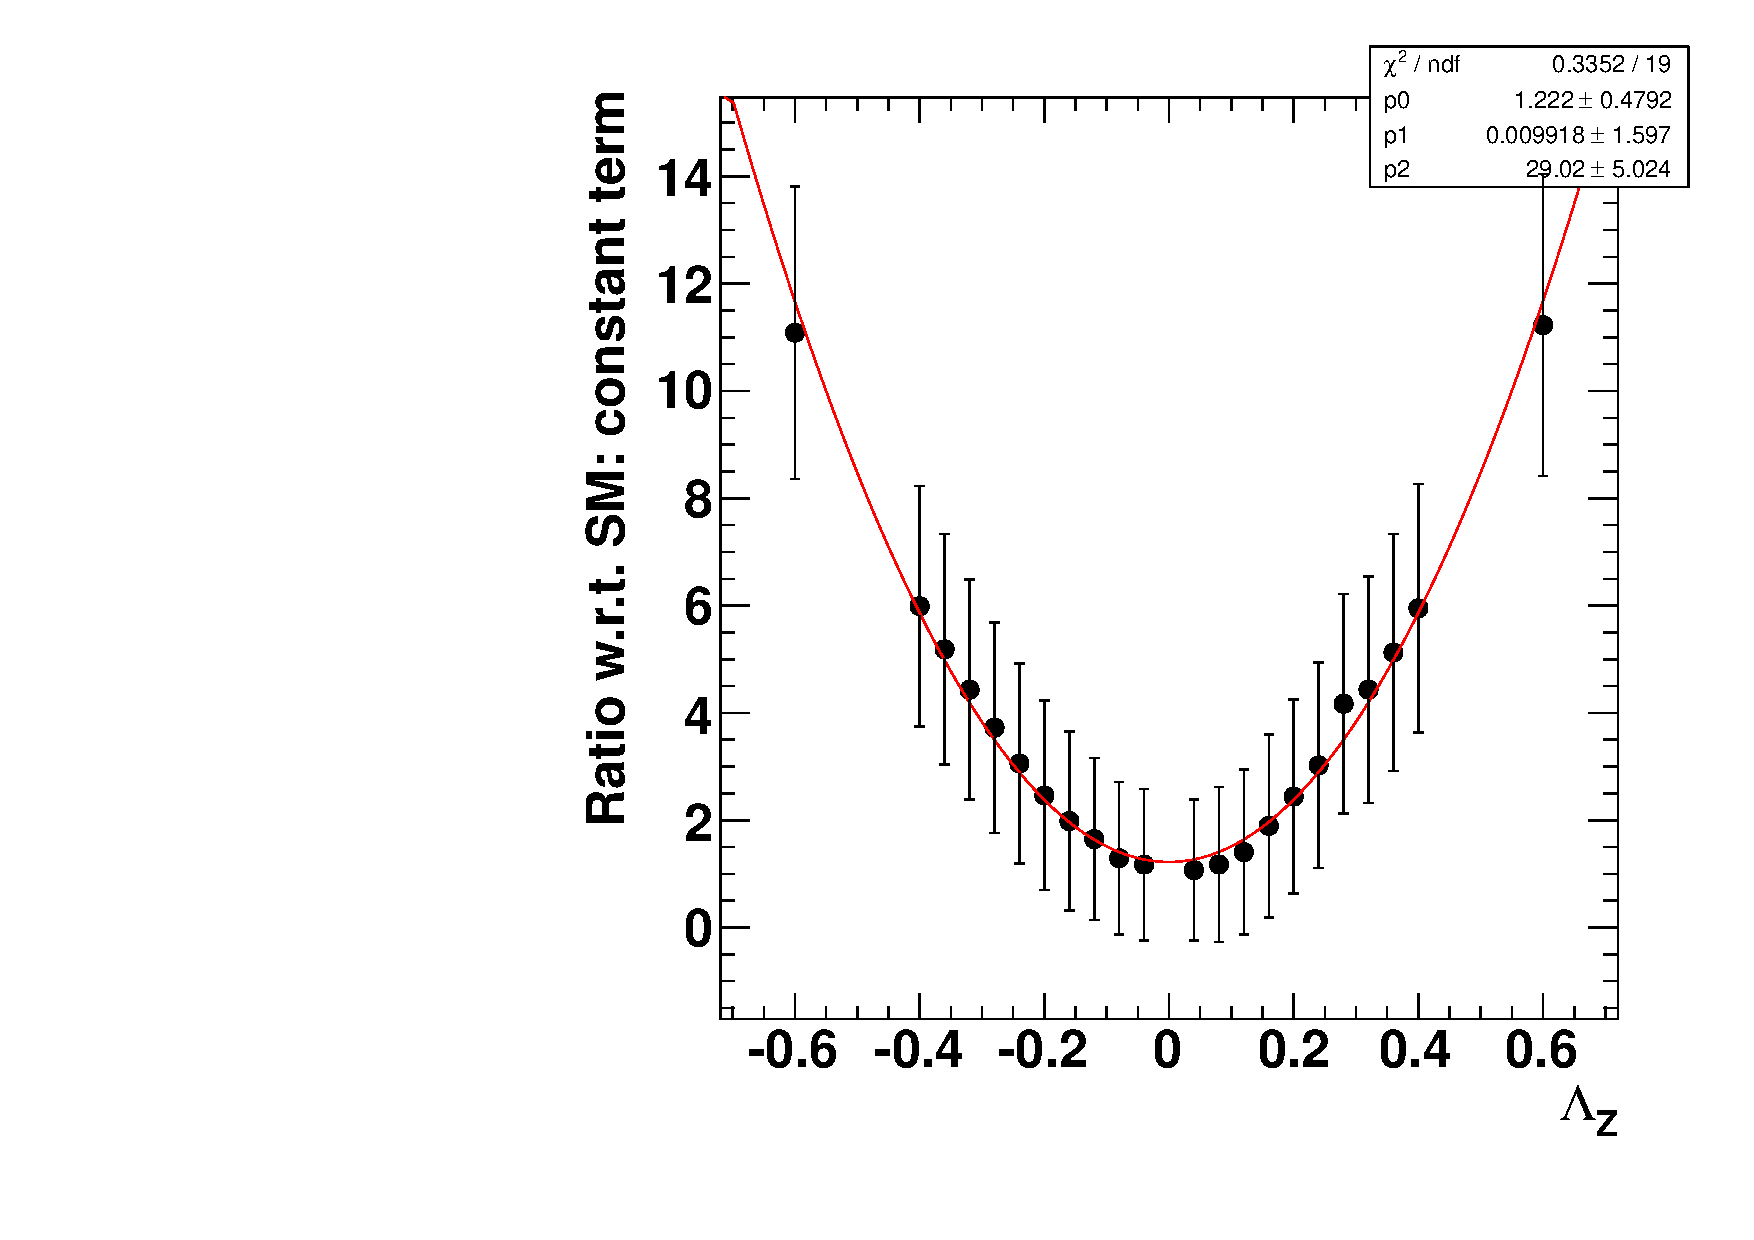
\includegraphics[width=0.32\textwidth]{figs/graphLambdaZP0.pdf}
    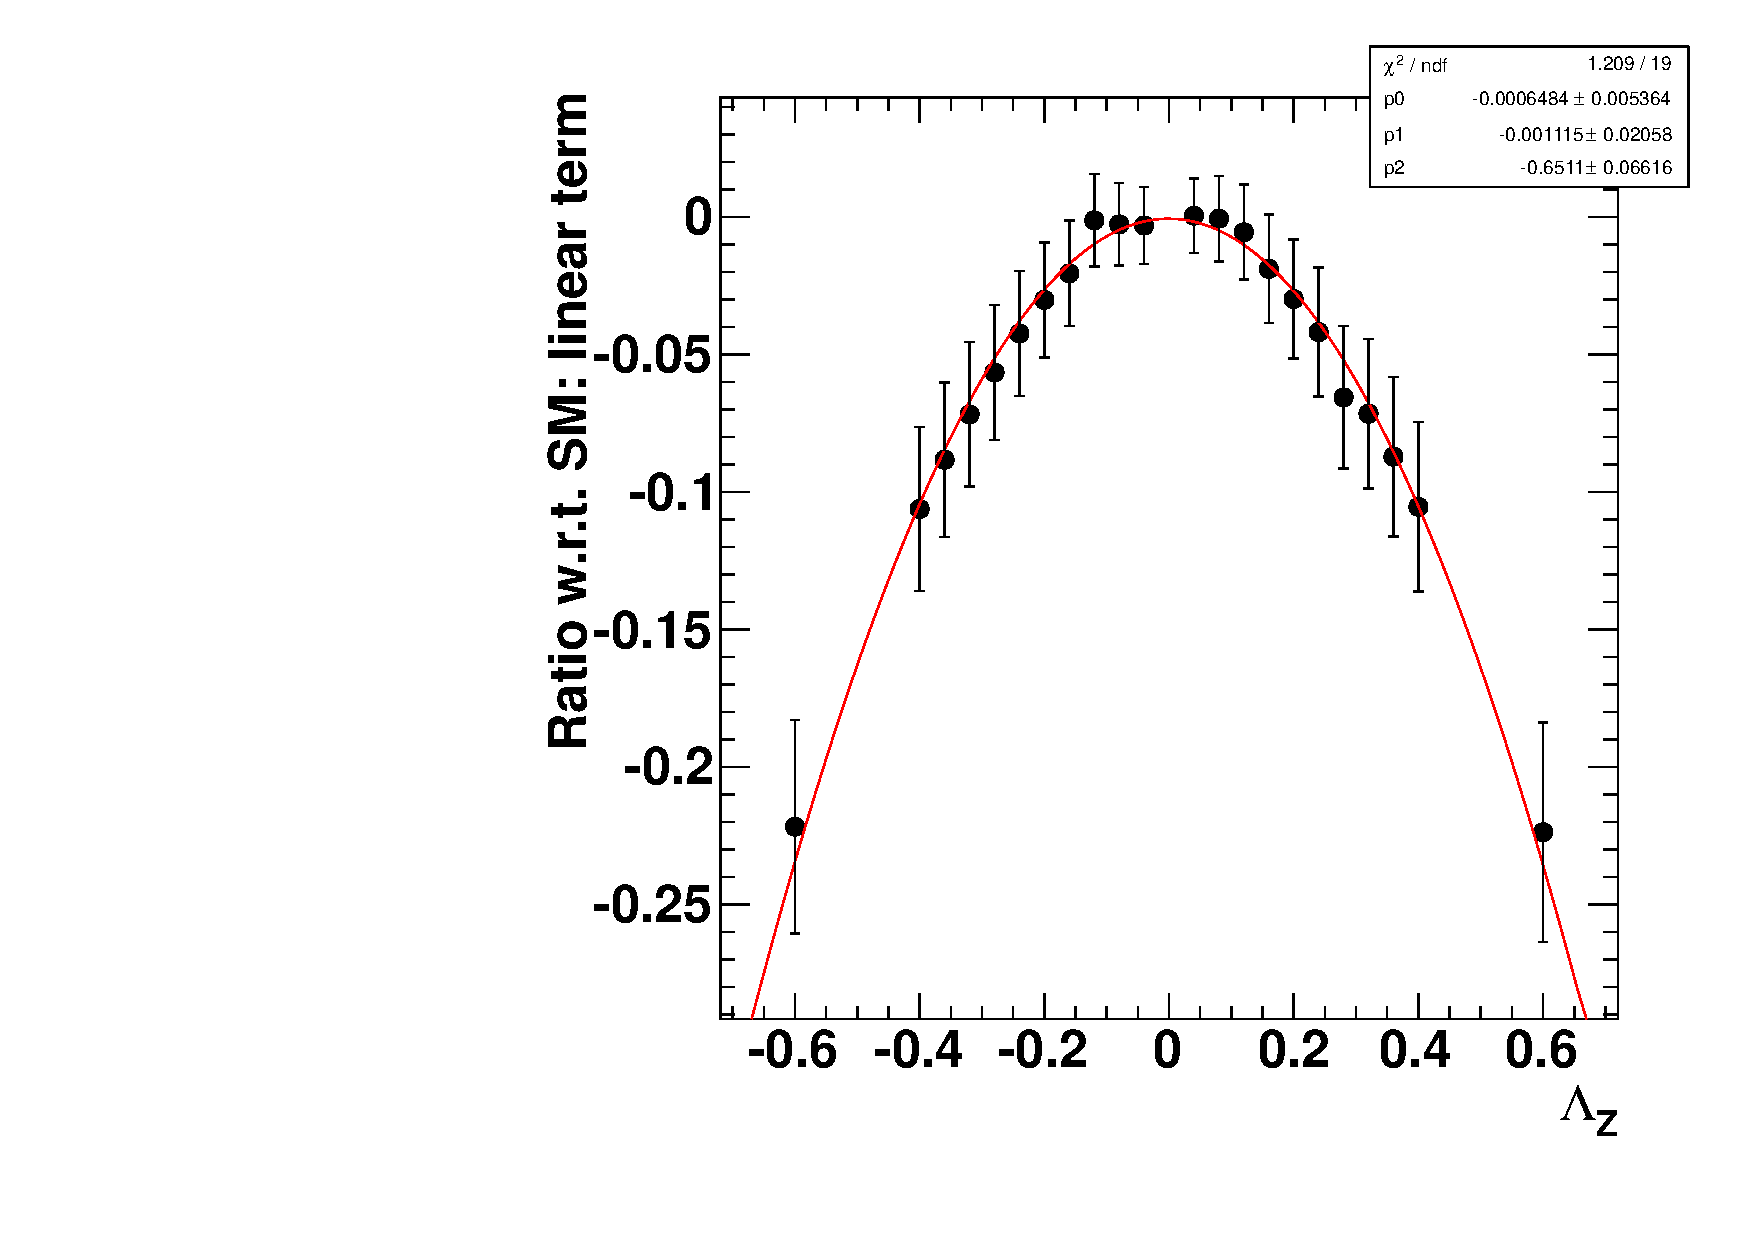
\includegraphics[width=0.32\textwidth]{figs/graphLambdaZP1.pdf}
    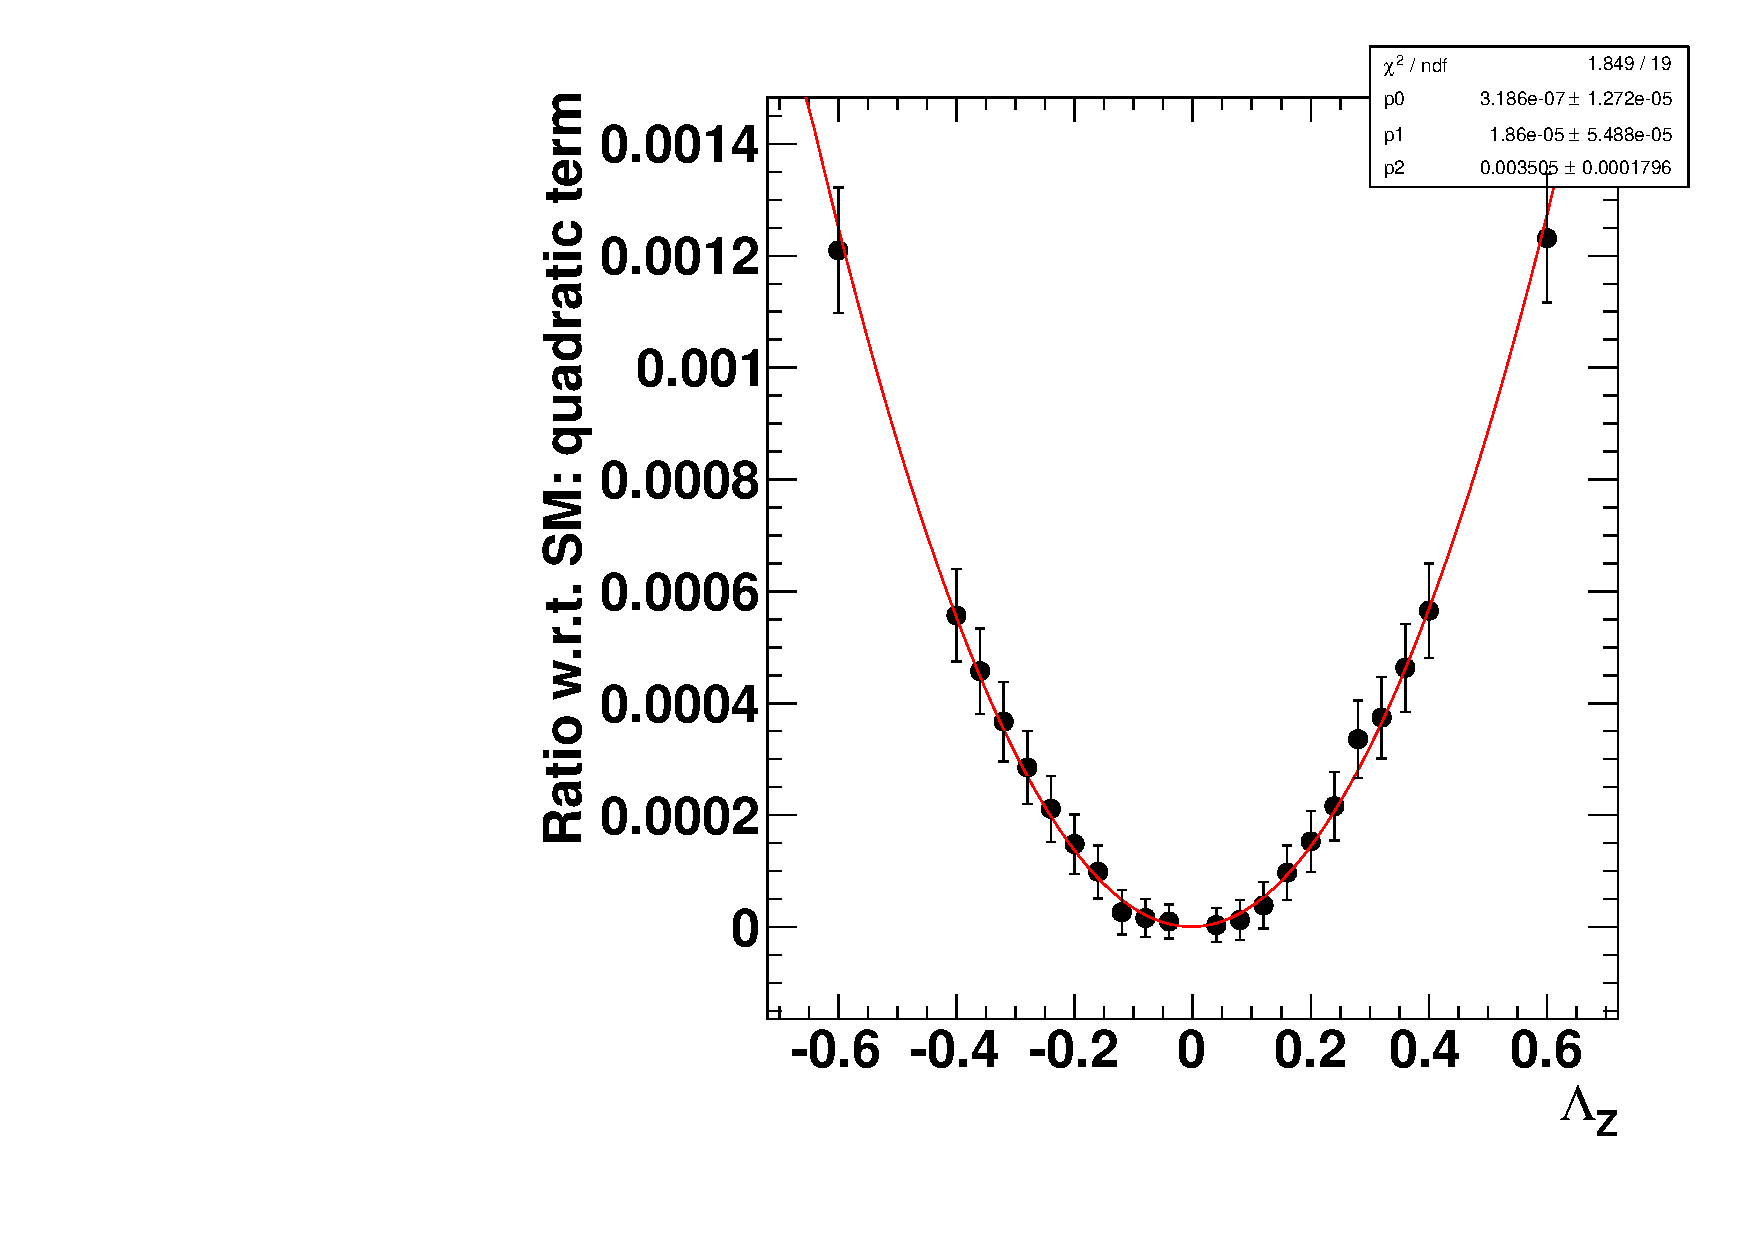
\includegraphics[width=0.32\textwidth]{figs/graphLambdaZP2.pdf}
    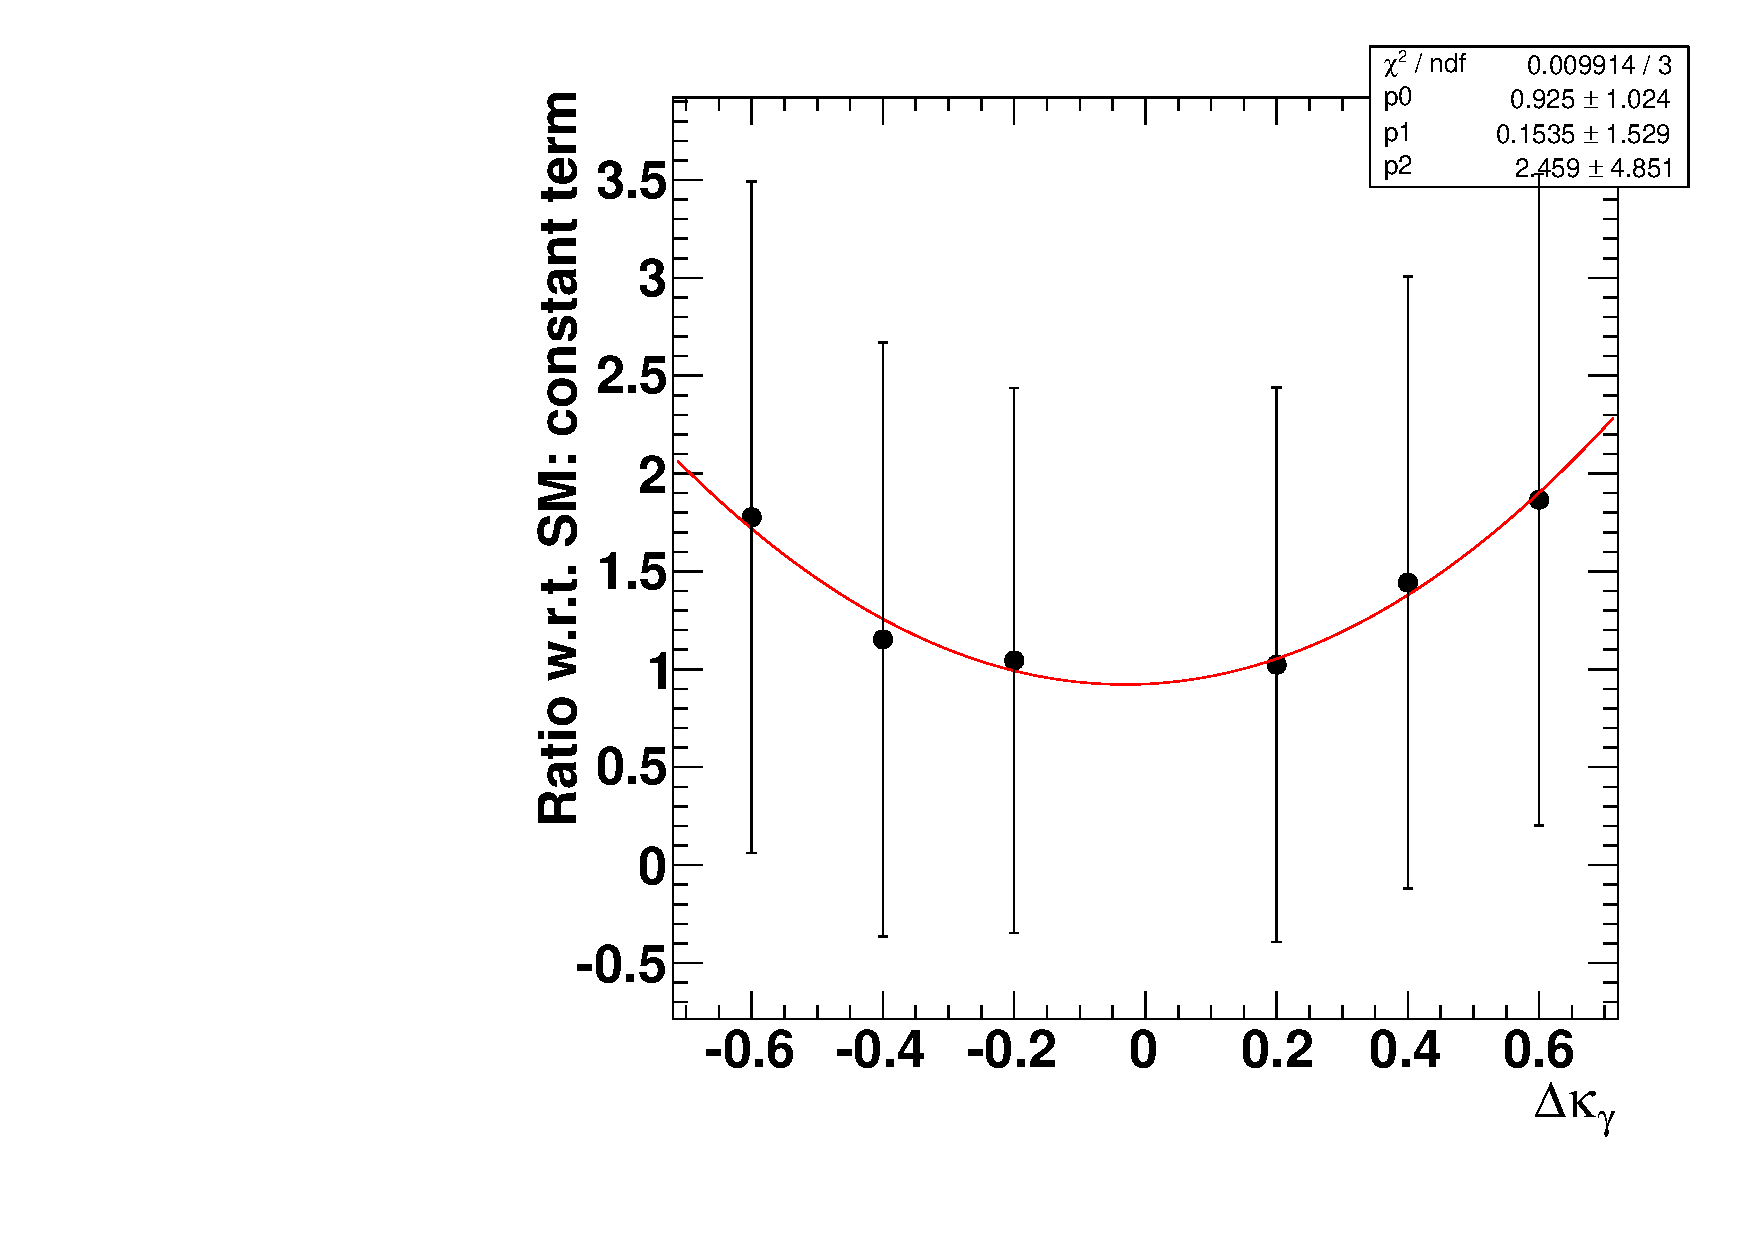
\includegraphics[width=0.32\textwidth]{figs/graphKappaGP0.pdf}
    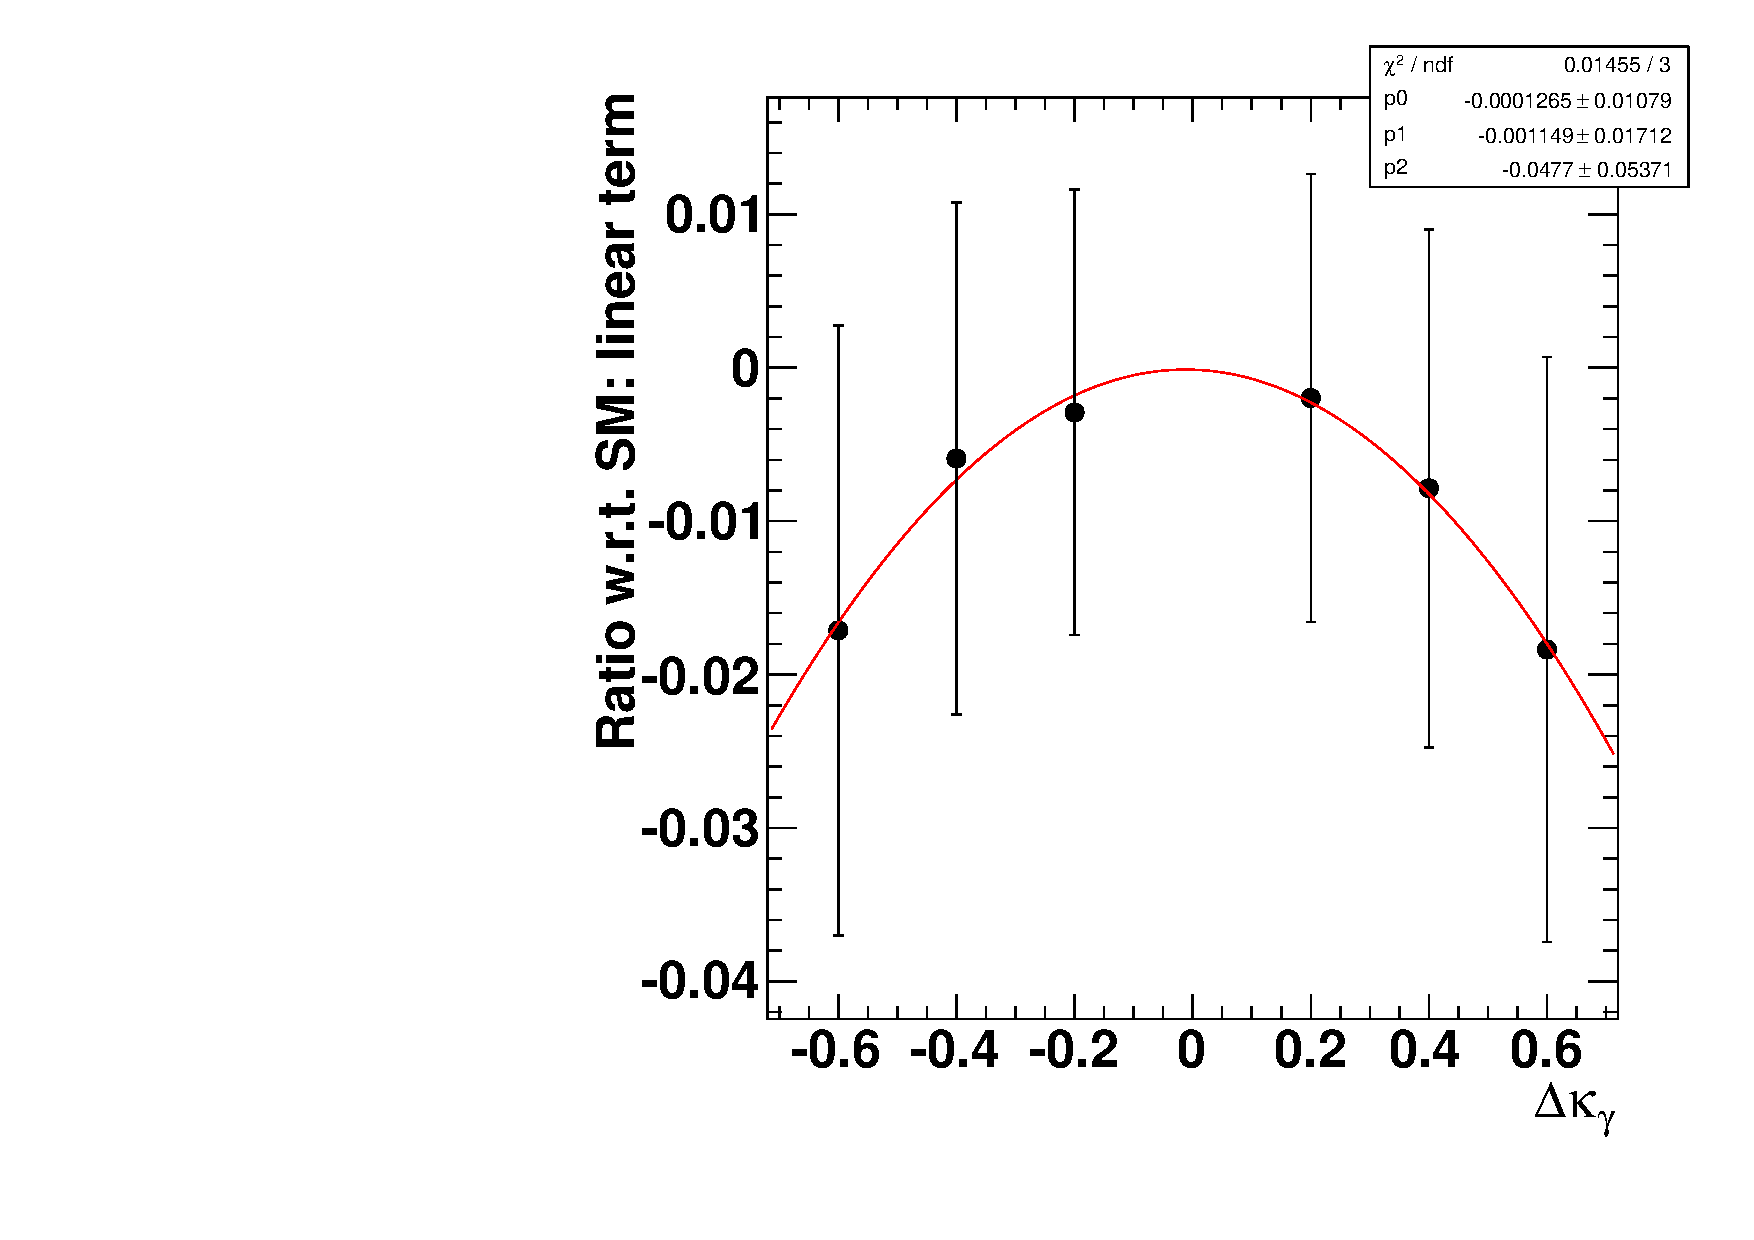
\includegraphics[width=0.32\textwidth]{figs/graphKappaGP1.pdf}
    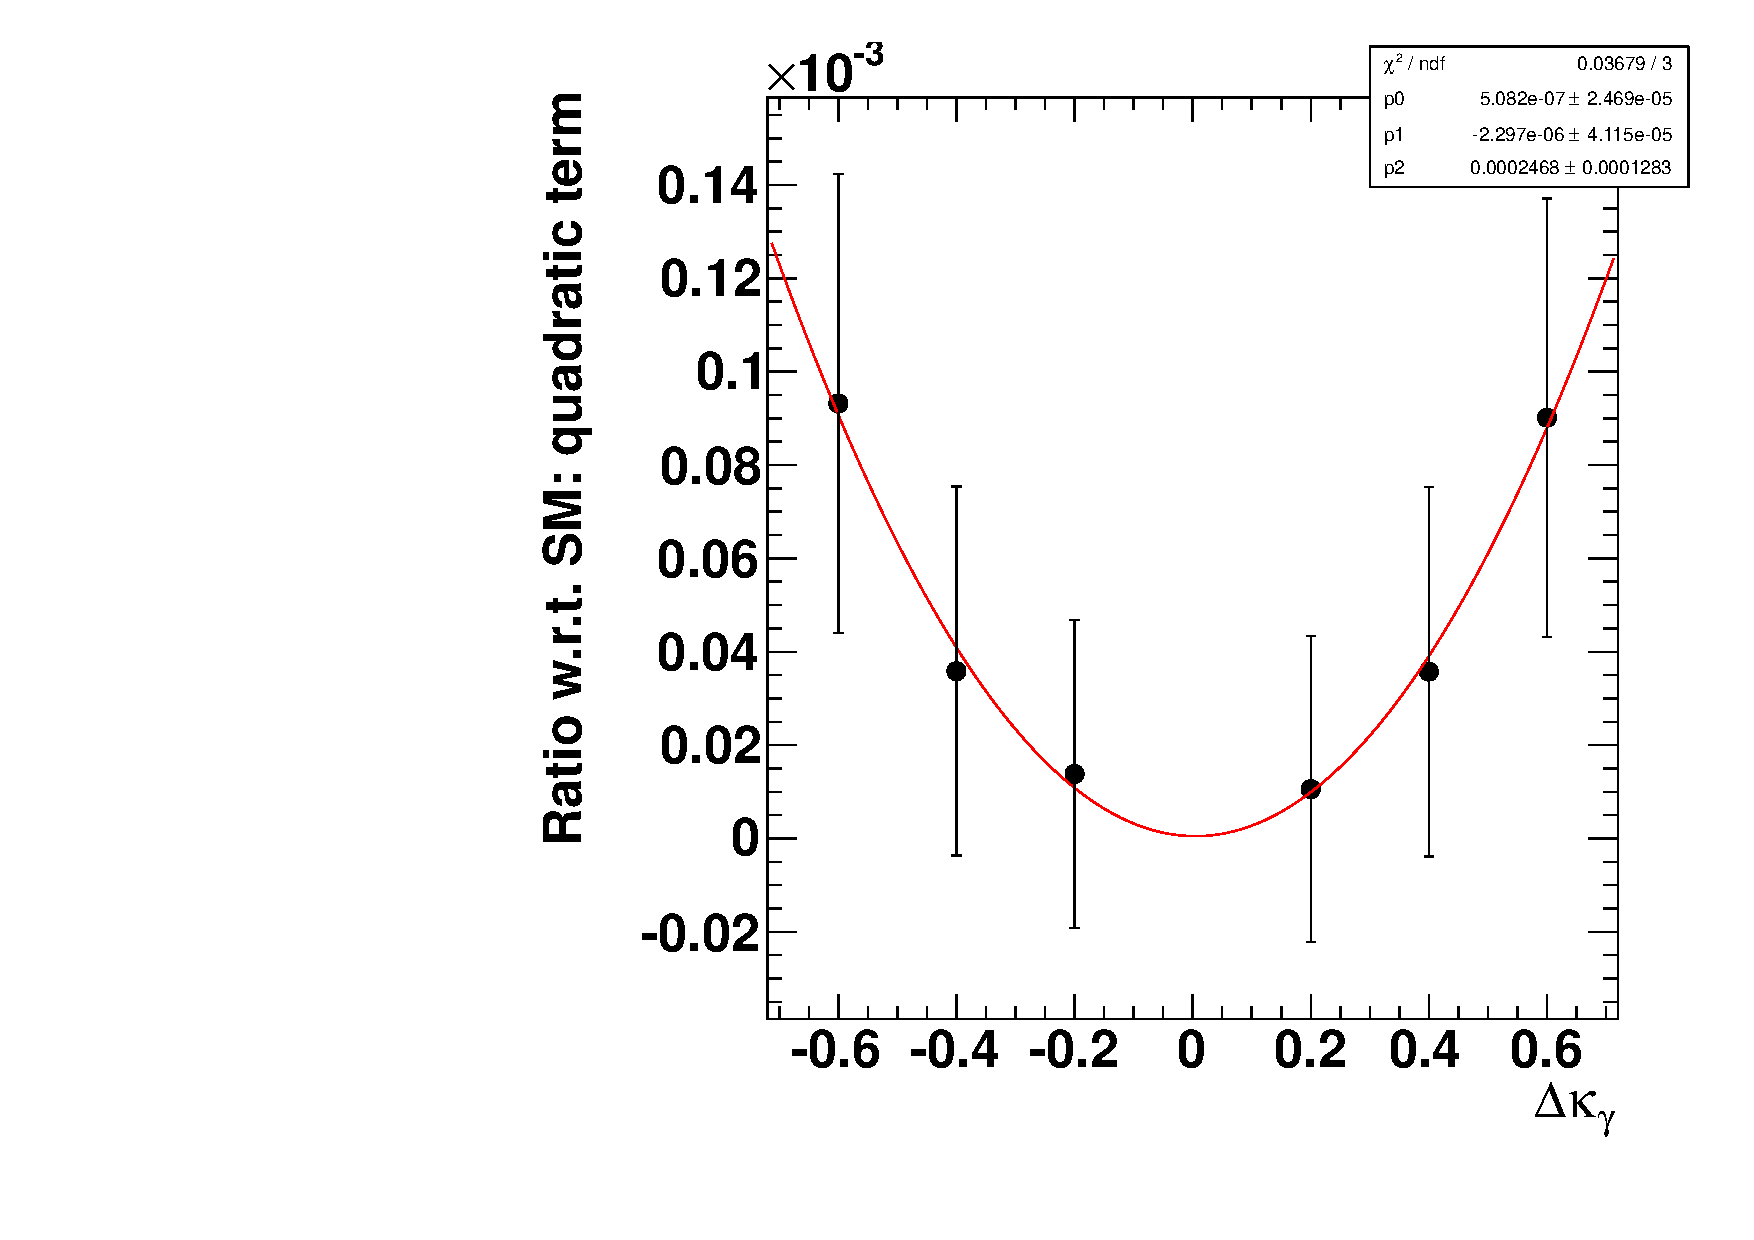
\includegraphics[width=0.32\textwidth]{figs/graphKappaGP2.pdf}
    \caption{Parametrization of $\Lambda_Z$ (top) and 
      $\Delta{\kappa_\gamma}$ (bottom).}
    \label{fig:aTGC_parametrization}}
\end{figure}
%%%%%%%%%%%%%%%%%%%%%%%%%%%%
%%%%%%%%%%%%%%%%%%%%%%%%%%%%


\begin{verbatim}
****************************************
lambdaZ: constant term
Chi2                      =     0.335214
NDf                       =           19
a0                        =      1.22156   +/-   0.479164    
a1                        =   0.00991771   +/-   1.59716     
a2                        =      29.0185   +/-   5.02385     

****************************************
lambdaZ: linear term
Chi2                      =      1.20931
NDf                       =           19
a0                        = -0.000648402   +/-   0.00536374  
a1                        =  -0.00111502   +/-   0.0205769   
a2                        =    -0.651108   +/-   0.0661579   


****************************************
lambdaZ: quadratic term
Chi2                      =      1.84914
NDf                       =           19
a0                        =  3.18629e-07   +/-   1.2723e-05  
a1                        =  1.85972e-05   +/-   5.48842e-05 
a2                        =   0.00350468   +/-   0.000179611 

****************************************
deltaKappaGamma: constant term
Chi2                      =   0.00991388
NDf                       =            3
a0                        =      0.92496   +/-   1.02405     
a1                        =     0.153547   +/-   1.52898     
a2                        =      2.45856   +/-   4.8514      

****************************************
deltaKappaGamma: linear term
Chi2                      =    0.0145474
NDf                       =            3
a0                        = -0.000126518   +/-   0.0107917   
a1                        =  -0.00114869   +/-   0.0171223   
a2                        =   -0.0477005   +/-   0.0537106   

****************************************
deltaKappaGamma: quadratic term
Chi2                      =    0.0367892
NDf                       =            3
a0                        =   5.0817e-07   +/-   2.46895e-05 
a1                        = -2.29715e-06   +/-   4.11536e-05 
a2                        =  0.000246789   +/-   0.000128328 
\end{verbatim}
%%%%%%%%%%%%%%%%%%%%%%%%%%%%%%%%%
